\documentclass[10pt]{beamer}
% adaptation au français et accents
\usepackage[utf8]{inputenc}
\usepackage[T1]{fontenc}

% insérer des images et graphiques
\usepackage{graphicx}
%video
\usepackage{media9}



%Thème
%\usetheme{Warsaw}
% couleurs
\usepackage{xcolor}
%theme de ses morts

%pour les numeros de pages
\addtobeamertemplate{footline}{\hspace{1em}\small\insertframenumber/\inserttotalframenumber}
%##########################################################

\begin{document}

\title{\huge Projet Scientifique Informatique}
	\subtitle{\Large L2 Informatique \\
	Modèle d'évacuation en cas urgence  }
	\author {Romain Kugler \& Yann Martin D'Escrienne}
	\institute{\normalsize Université Nice-Sophia Antipolis}
	\date{2019}
	
%Affiche le titre ci-dessus	
\begin{frame} \titlepage \end{frame}

%Intro
\begin{frame}
	\frametitle{\textbf {\Large Introduction}}
	\framesubtitle{\large Contexte}
	
	\begin{block}{}
	\begin{itemize}
		\item \textbf{De quoi s'agit-il ?} \\
		Modélisation d'évacuation en cas d'urgence\\
		\item \textbf{Qui ?}\\
		Individus de tous âges et milieux sociaux \\
		\item \textbf{Où ?}\\
		Salle de cinéma, amphithéâtre, bureaux...\\
		\item \textbf{Quels dangers ?}\\
		Feu, Attentats, Fumée...
	\end{itemize}
	\end{block}	
\end{frame}



%Problématique
\begin{frame}
	\frametitle{\textbf {\Large Introduction}}
	\framesubtitle{\large Enjeux}
	
	\begin{block}{\textbf{Quels enjeux?}}
	\begin{itemize}
		\item Limiter les pertes humaines
		\item Optimiser l'évacuation 	
	\end{itemize}
	\end{block}
	
	\medskip
	
	\begin{block}{\textbf{Pour cela il faut :}}
	\begin{itemize}
		\medskip
		\item Identifier les paramètres importants d'une évacuation
		\smallskip 
		\item Obtenir un temps d'évacuation minimal\\
		\smallskip 
		\item Des conditions qui limitent le nombre de décès
	\end{itemize}
	\end{block}
	
	
\end{frame}

\begin{frame}
	\frametitle{\textbf {\Large Questions scientifiques :}}
	\begin{center}
		\LARGE \textcolor{red}{\textbf {Comment optimiser une évacuation?}}
	\end{center}
		
	\medskip 
	\large \textbf{Autrement dit :} 	
	\medskip
	
	\begin{itemize}
		\item \large Quelle est l'influence des paramètres sur l'efficacité de l'évacuation ?
		\medskip
		\item \large A quel endroit le danger est-il le plus important ?
	\end{itemize}
		
	
	
\end{frame}

%Modélisation


\begin{frame}
	\frametitle{\textbf {\Large Modélisation}}
	\framesubtitle{\large Description du modèle}
	\begin{block}{\textbf{Paramètres}}
	\begin{enumerate}
		\item \textbf{Densité} d'individus dans la salle\\
		\item Nombre de \textbf{sorties}\\
		\item \textbf{Obstacle} devant la sortie \\
		\item Emplacement du \textbf{feu}\\
	\end{enumerate}
	\end{block}
	
	
	\begin{block}{\textbf{Mesures}}
	\begin{enumerate}
		\item \textbf{Temps moyen} d'évacuation\\
		\item \textbf{Nombre d'individus} évacués au temps T\\
		\item \textbf{Nombre de décès} lors de l'incendie\\
	\end{enumerate}
	\end{block}
\end{frame}



\begin{frame}
	\frametitle{\textbf {\Large Modélisation}}
	\begin{block}{\textbf{Hypothèses simplificatrices}}
	\medskip
	\begin{itemize}
		\item Monde en 2D
		\medskip 
		\item Feu, sièges, obstacles,.. occupent une case
		\medskip 
		\item Les individus ont la même vitesse de déplacement
		\medskip 
		\item Ils ont la même taille
		\medskip 
		\item Ils ne peuvent pas se pousser
	\end{itemize}
	\end{block}
\end{frame}


\begin{frame}
	\frametitle{\textbf {\Large Simulation}}
	\begin{figure}
				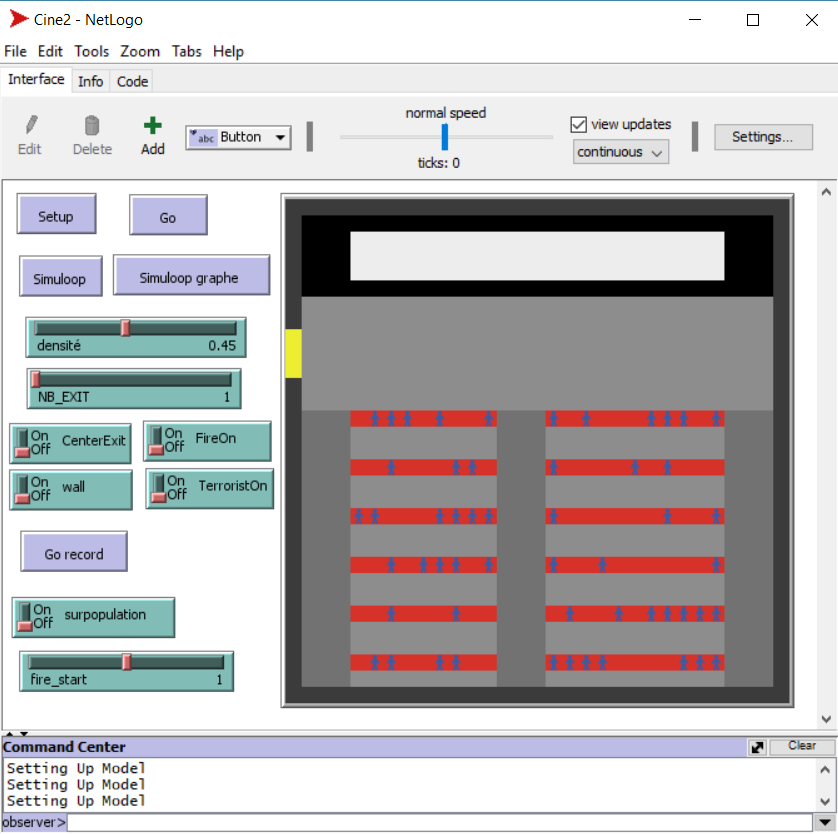
\includegraphics[scale=0.45]{capture.PNG}
 				\label{pic: capture}
 			\end{figure}
\end{frame}


\begin{frame}
	\frametitle{\textbf {\Large Simulation}}
	\framesubtitle{\large Cadre expérimental}
	\begin{itemize}
		\item Salle de cinéma de dimension 30x30
		\medskip 
		\item Déplacement intelligent des turtles\\
		\medskip
		\small (contournement, sortie la plus proche,\\réaction en fonction de ses voisines)
		\medskip
		\item Évacuation effectuée une fois la sortie atteinte
		\medskip
		\item Propagation du feu selon une probabilité
	\end{itemize}
\end{frame}

\begin{frame}
	\frametitle{\textbf {\Large Simulation}}
	\framesubtitle{\large Protocole expérimental}
	\begin{enumerate}

		\item Faire varier le nombre de sorties et mesurer le nombre \\d'évacués au temps T de chaque cas. 
		\medskip 
		\item Faire varier la densité et mesurer le temps d'évacuation \\de chaque cas. 
		\medskip 
		\item Changer l'emplacement du feu et mesurer la répartition \\du nombre de morts. 
		\medskip 
		\item Créer une surpopulation sur une sortie et calculer la moyenne \\du temps d'évacuation avec et sans obstacle.
		\medskip 
	\end{enumerate}

\end{frame}

\begin{frame}
 	\frametitle{\textbf {\Large Résultats: Nombre de sorties}}
 	\begin{columns}
 	 	
 	 	\column{0.5\textwidth}
 	 		\begin{figure}
     		 \begin{tikzpicture}[remember picture,overlay]
         		\node[anchor=west, inner sep=3pt] at (current page.west) {%
          		 \includemedia[
           		  addresource=1sortie.mp4,
           		  activate=pageopen,transparent,
          		   flashvars={
          		   source=1sortie.mp4},
	             width=0.5\paperwidth,height=0.5\paperheight
         		  ]{}{VPlayer.swf}%
        		 };
     		 \end{tikzpicture}
     		 \end{figure}
     	\column{0.5\textwidth}
     		\begin{figure}
     		 \begin{tikzpicture}[remember picture,overlay]
         		\node[anchor=east, inner sep=3pt] at (current page.east) {%
          		 \includemedia[
           		  addresource=2sortie.mp4,
           		  activate=pageopen,transparent,
          		   flashvars={source=2sortie.mp4},
	             width=0.5\paperwidth,height=0.5\paperheight
         		  ]{}{VPlayer.swf}%
        		 };
     		 \end{tikzpicture}
     		\end{figure}
 	
 	\end{columns}
      

\end{frame}

\begin{frame}
	\frametitle{\textbf {\Large Résultats}}
	\framesubtitle{\normalsize Nombre de sorties}
		\begin{columns}

		\column{0.45\textwidth}
			\begin{figure}
				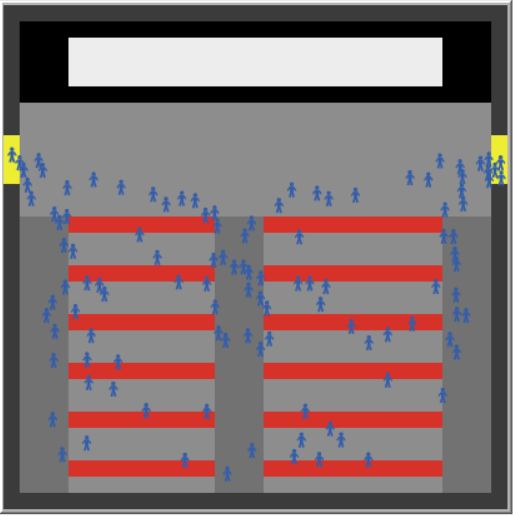
\includegraphics[width=\linewidth]{Capture_sortie.PNG}
 				\label{pic: sortie}
 			\end{figure}

		\column{0.52\textwidth}
				\begin{figure}
				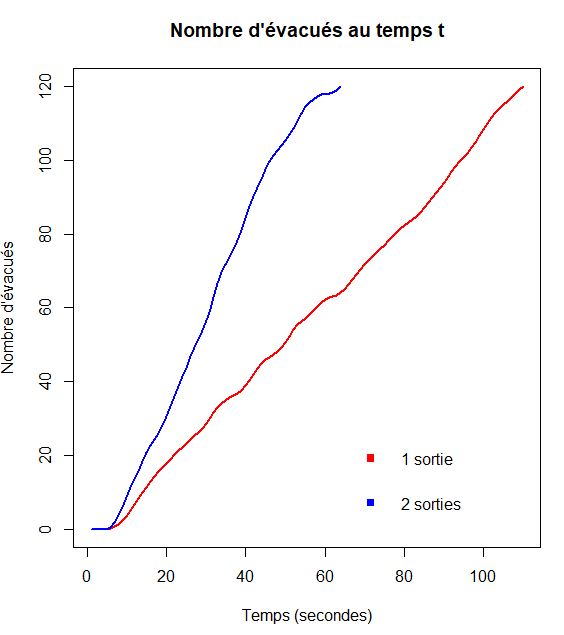
\includegraphics[width=\linewidth]{nb_sortie.PNG}
 				\caption{Temps selon le nombre de sorties}
 				\label{pic: sortie2}
 			\end{figure}
	\end{columns}
\end{frame}



\begin{frame}
	\frametitle{\textbf {\Large Résultats}}
	\framesubtitle{\normalsize Densité}
	\begin{columns}

		\column{0.55\textwidth}
			\begin{figure}
				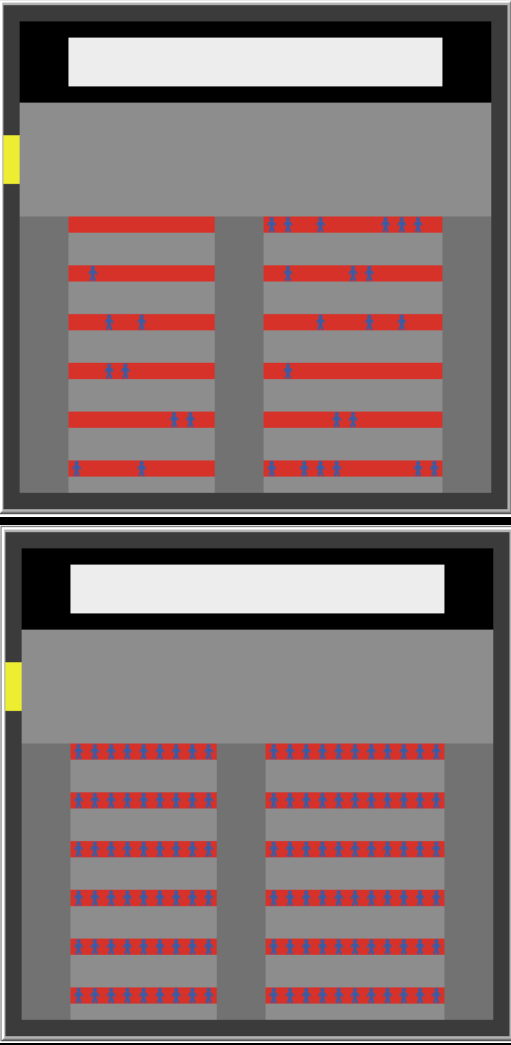
\includegraphics[scale = 0.35]{capture_densite.PNG}
 		
 				\label{pic: densite}
 			\end{figure}

 

		\column{0.55\textwidth}
			\begin{figure}
				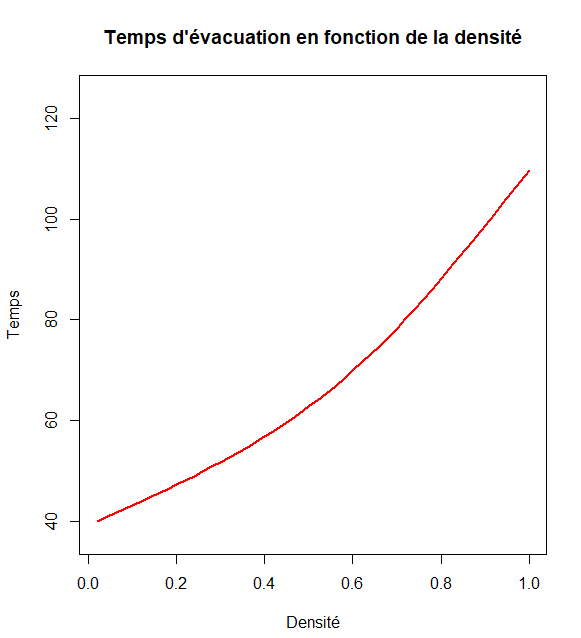
\includegraphics[scale = 0.28]{densite_temps.PNG}
 				\caption{Temps en fonction de la densité}
 				\label{pic: densite2}
 			\end{figure}

	\end{columns}

	

\end{frame}

\begin{frame}
 	\frametitle{\textbf {\Large Résultats: Départ du feu}}
      \begin{tikzpicture}[remember picture,overlay]
         \node[anchor=north west, inner sep=30pt] at (current page.north west) {%
           \includemedia[
             addresource=feu.mp4,
             activate=pageopen,transparent,
             flashvars={source=feu.mp4},
             width=0.85\paperwidth,height=0.85\paperheight
           ]{}{VPlayer.swf}%
         };
      \end{tikzpicture}

\end{frame}

\begin{frame}
	\frametitle{\textbf {\Large Résultats}}
	\framesubtitle{\normalsize Départ du feu}
	
	\begin{center}
	\textbf{\normalsize Sur 20 simulations : }
	\end{center}
	
	\begin{columns}

		\column{0.45\textwidth}
			\begin{figure}
				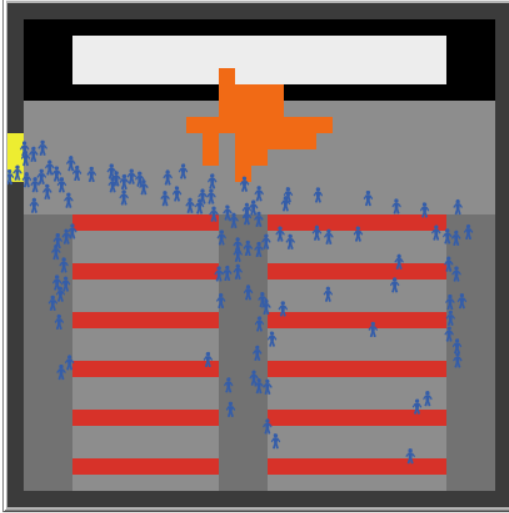
\includegraphics[width=\linewidth]{capture_feu.PNG}
 				\label{pic: feu}
 			\end{figure}
 
		\column{0.49\textwidth}
			\begin{figure}
				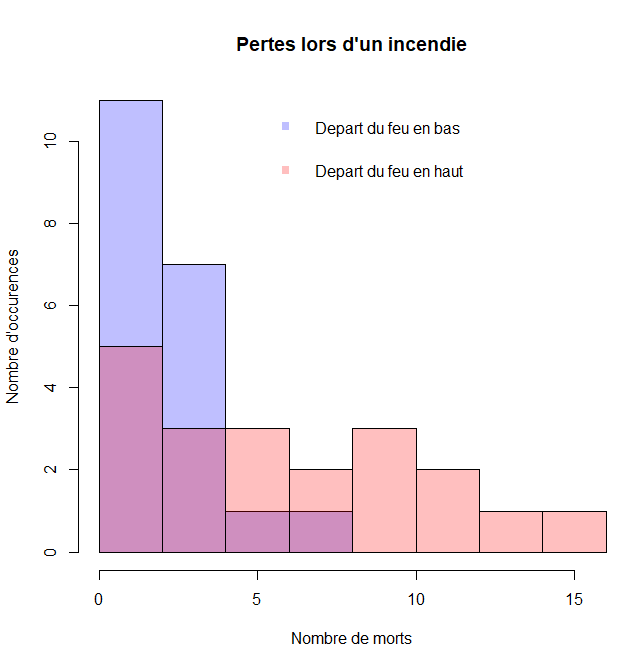
\includegraphics[width=\linewidth]{graphe_nb_mort.PNG}
 				\caption{Répartition du nombre de morts selon le départ du feu}
 				\label{pic: feu2}
 			\end{figure}

	\end{columns}
	
\end{frame}

\begin{frame}
 	\frametitle{\textbf {\Large Résultats: Obstacle}}
 	\begin{columns}
 	 	
 	 	\column{0.5\textwidth}
 	 		\begin{figure}
     		 \begin{tikzpicture}[remember picture,overlay]
         		\node[anchor=west, inner sep=3pt] at (current page.west) {%
          		 \includemedia[
           		  addresource=sansobstacle.mp4,
           		  activate=pageopen,transparent,
          		   flashvars={
          		   source=sansobstacle.mp4},
	             width=0.5\paperwidth,height=0.5\paperheight
         		  ]{}{VPlayer.swf}%
        		 };
     		 \end{tikzpicture}
     		 \end{figure}
     	\column{0.5\textwidth}
     		\begin{figure}
     		 \begin{tikzpicture}[remember picture,overlay]
         		\node[anchor=east, inner sep=3pt] at (current page.east) {%
          		 \includemedia[
           		  addresource=obstacle.mp4,
           		  activate=pageopen,transparent,
          		   flashvars={source=obstacle.mp4},
	             width=0.5\paperwidth,height=0.5\paperheight
         		  ]{}{VPlayer.swf}%
        		 };
     		 \end{tikzpicture}
     		\end{figure}
 	
 	\end{columns}
      

\end{frame}

\begin{frame}
	\frametitle{\textbf {\Large Résultats}}
	\framesubtitle{\normalsize Obstacle}
	
	\begin{center}
	\textbf{\normalsize Sur 20 simulations : }
	\end{center}
	
	
	\begin{columns}

		\column{0.55\textwidth}
			\begin{figure}
				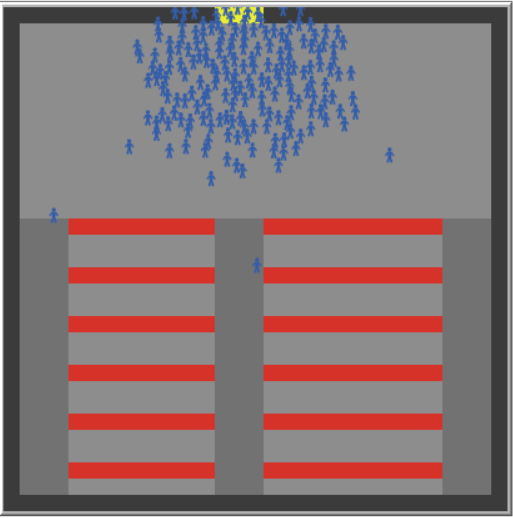
\includegraphics[scale = 0.35]{capture_sans_obstacle.PNG}
				\caption{Sans obstacle}
 		
 				\label{pic: obstacle}
 			\end{figure}
		\hspace{4em}\textbf{Moyenne : 224.7}
 

		\column{0.55\textwidth}
			\begin{figure}
				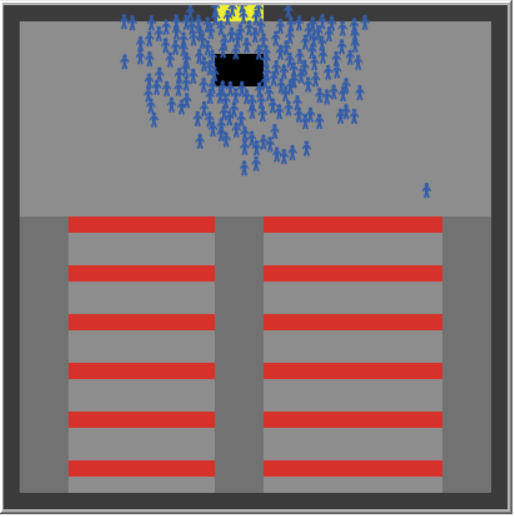
\includegraphics[scale = 0.35]{capture_obstacle.PNG}
 				\caption{Avec obstacle}
 				\label{pic: obstacle2}
 			\end{figure}
 			
 		\hspace{4em}\textbf{Moyenne : 213.75}

	\end{columns}
	
	
	



\end{frame}

\begin{frame}
	\frametitle{\textbf {\Large Conclusion}}
	\framesubtitle{\large Déduire des résultats expérimentaux}
	\begin{block}{\textbf {\large Répondre aux problèmes posés}}
	\medskip
		\begin{enumerate}
			\item Nombre et emplacements judicieux des sorties 
			\medskip
			\item Limiter la capacité maximale d'une salle 
			\medskip
			\item Disposition optimale des extincteurs
			\medskip
			\item Ajout d'un obstacle séparateur devant les sorties importantes
			
		\end{enumerate}
	\end{block}
%		\includemedia[
%		width = 3cm, height = 3cm,
%		addresource=1sortie.mp4,
%		passcontext,
%		activate=pageopen,
%		flashvars={
%		source=1sortie.mp4,
%		&loop=true,
%		&autoplay=true
%		}]{\fbox{Click!}}{APlayer.swf}
\end{frame}

\begin{frame}
	\frametitle{\textbf {\Large Limites du modèle}}
	\begin{block}{}
		\medskip
		\begin{itemize}
			\item \large Possibilité d'un meilleur effet de congestion
			\medskip
			\item \large Feu plus réaliste 
			\medskip
			\item \large Prise en compte de l'âge des individus (vitesse et taille)
			\medskip
			\item Autres dispositions de la salle
		\end{itemize}
	\end{block}

\end{frame}


\end{document}
